\documentclass[a4paper,10pt]{article}
\usepackage{graphicx}
\usepackage[english]{babel}
\usepackage[latin1]{inputenc}

\usepackage{listings}
\usepackage{geometry}
\usepackage{float}
\usepackage{amsmath,amsthm}
\usepackage{amsfonts}
\usepackage{amssymb}
\usepackage{caption}
\usepackage{subcaption}
%
\begin{document}
%
   \title{Math 483 Project}

   \author{Jesus Banuelos, Elizabeth Duran, Benjamin Bonilla, Salvador Tamayo \\ Ling - MATH 483 }
          
   \date{May 21, 2021}

   \maketitle
   
   \tableofcontents
 
   \newpage
\addcontentsline{toc}{section}{Abstract}
\begin{abstract}
Concepts of mathematical modeling and the biological phenomenon of population
growth rate models can be utilized for investigating the stability of a species
population. Replicating results of previous publications of rapid declining
population models through different computer programming languages such as MATLAB
verify the mathematical model's practical implementation and population growth
rate prediction accuracy. The general purpose of the study is to show that if a
honeybee model from the research works presented in this study can be replicated
and its results of the model are the same, then this confirms a measure of the
likelihood of a mathematical model repeatability and verifies the results are
true and not by chance.
\end{abstract}
\section{Introduction}

\subsection{Mathematical Problem}
Honeybee population growth models can be developed to analyze the honeybee
species' historic rapid population decline reportedly since 2006 \cite{Nowrski}. There are
many factors that can contribute to the death of a honeybee colony such as
diseases, predators, nutrition shortages, pesticides, environmental pollutants,
environmental loss, climate variability, agricultural practices, reduced total
number of species genetic characteristics, and Colony Collapse Disorder (CCD). To
compartmentalize these factors in a model can be impractical and result in
overfitting. A mathematical model of the Honeybee colony population decline has
been developed by David S. Khoury, Mary R. Myerscough, and Andrew B. Barron \cite{Kho}
represented by two differential equations that model the hive honeybee and
forager honeybee populations interaction and the forager honeybee death rate
impact on a honeybee colony decline. This model from Khoury, Myerscough, and
Barron has been extended by Kelly Brown of the University of Mary Washington.
Brown implemented a ``Mathematica Demonstration code that [allows manipulation]
of the hive bee and forager per capita death rates as well as a reflection of
brood mortality to create Phase Plane Diagrams for [the mathematical] model [of
honeybee populations] on a custom scale'' \cite{Brown}. The extended mathematical model of
honeybee populations depends on the consideration of a hive honeybee death rate.
To understand the importance of the hive honeybee and forager honeybee
interaction and death rates in a mathematical model their biological traits and
behavior must be explained.

\subsection{Biological Background}
Biological traits and behaviors of the honeybee are distinct depending on the
following different types: Worker, Drone, and Queen. The Worker female bees can
forage for sustenance and create the bee nest (beehive) through secreting beeswax
and shaping it into a hexagonal cell structure. The hexagonal structures contain
capped honeycomb cells for pollen and honey or broodcomb cells where the Queen
female bee lays eggs, which eventually develops into larva then a pupa, before
transitioning into an adult and escaping the cell. A brood is essentially the
young offspring of a Queen bee and is nursed by Worker bees. Queen bees mainly
lay eggs and produce pheromones that assist in controlling colony reproduction
and colony social organization. Drone male bees only assist in the reproduction
of bees through mating with the Queen bee in the hive, otherwise they are not
allowed in the beehive.\\
The two types of Worker honeybees are Hive bees and Forager bees. Social
inhibition in Worker bees is essentially when Forager bees of the beehive stop
the transition from foraging by feeding the younger hive bees which delays the
conversion to foragers. An absence of hive bees will prompt foragers to
revert to being a hive bee \cite{Brown}. Alternatively, a decrease in forager bees will
prompt younger hive bees to become foragers earlier, known as precocious foraging
\cite{Brown}. If there was an absence of all Hive bees and Forager bees, then the whole
population of a honeybee colony would fail with other types of bees not being
able to feed themselves. Hive bees and Forager bees are the main components to
determine a population rate of a honeybee colony since Drone bees do not
contribute any sustenance.

\section{Model}
The Khoury, Myerscough, Barron and Brown models display different factors on colony failures by differential equations. The model differs two different equations that describe the interaction between the hive bee and forager bee populations. \\
Equation 1: The Khoury, Myerscough, and Barron
\begin{displaymath}
	\frac{dH}{dt} = \frac{L(H+F)}{(\omega +H+F)} - H(\alpha - \sigma (\frac{F}{H+F}))
\end{displaymath}
\begin{displaymath}
	\frac{dF}{dt} = H(\alpha - \sigma (\frac{F}{H+F})) - mF
\end{displaymath}
Equation 2: Brown
\begin{displaymath}
	\frac{dH}{dt} = \frac{L(H+F)}{(\omega +H+F)} - H(\alpha - \sigma (\frac{F}{H+F})) - \mu H
\end{displaymath}
\begin{displaymath}
	\frac{dF}{dt} = H(\alpha - \sigma (\frac{F}{H+F})) - mF
\end{displaymath}
The first equation describes the rate of change of hive bee population which represents the emergence of the bees and then subtracts the bee population that transitions to foraging. In the equation, sigma represents the inhibition that is proportional to the number of foragers in the colony. $\mu$ is the parameter that is proportional to $\mu = km$ for a positive constant. Omega is the brood mortality, L is equal to the maximum laying rate of the queen, F is equal to the number of forager bees and m is equal to the death rate.
The Brown model equation is the equation we used to replicate the bee model which is where we used the parameter in order to distinguish the hive bee vs the foraging bee population.  
Although, the death rate for the beehives is set to be negligible. In order to proceed and find a solution we need to consider a parameter which leads us to find the balance between the hive bees and foragers since hive bees work longer. The two equations will be set equal to zero and will help us find the equilibrium. After we find the equilibriums, we then determine the global stability for each equilibrium found by applying the Jacobian Matrix. Then for stability we apply the trace is less than zero and determinant is greater than zero. Therefore, we can conclude where the bees are increasing or decreasing.

\section{Equilibrium}
In order to find the equilibrium points we will set $\frac{dH}{dt} = 0$ and $\frac{dF}{dt} = 0$ 
\begin{displaymath}
H(\alpha - \sigma (\frac{F}{H+F})) = mF
\end{displaymath}
and
\begin{displaymath}
\frac{L(H+F)}{(\omega +H+F)}-mF-kmH =0
\end{displaymath}
If we use the same technique that Brown used then $H = \frac{1}{J}F \rightarrow F = JH$ Therefore, $\frac{dH}{dt}$ turns into 
\begin{displaymath}
\frac{L(H+JH)}{(\omega +H+JH)}-mJH-kmH =0
\end{displaymath}
Which then turns into the following,
\begin{displaymath}
LH(1+J)=mH(J+k)(\omega + H(1+J))
\end{displaymath}
As you can see t he H terms cancel out leaving us with,
\begin{displaymath}
L(1+J)=m(J+k)(\omega + H(1+J))
\end{displaymath}
Now we expand and simplify,
\begin{displaymath}
L = \frac{mJ\omega +mk\omega}{1+J}+mJH+mkH
\end{displaymath}
Now by pulling out H and subtracting some terms we get, 
\begin{displaymath}
L - \frac{mJ\omega +mk\omega}{1+J}=H(mJ+mk)
\end{displaymath}
Then we isolate H and get,
\begin{displaymath}
\frac{L}{(mJ+mk)} - \frac{mJ\omega +mk\omega}{(1+J)(mJ+mk)}=H
\end{displaymath}
Now pull out $\omega$ and it gives us, 
\begin{displaymath}
\frac{L}{(mJ+mk)} - \frac{\omega(mJ +mk)}{(1+J)(mJ+mk)}=H
\end{displaymath}
Now we cancel out the $(mJ +mk)$
Now pull out $\omega$ and it gives us, 
\begin{displaymath}
H = \frac{L}{(mJ+mk)} - \frac{\omega}{(1+J)}
\end{displaymath}
Since $F=JH$ then 
\begin{displaymath}
F = J (\frac{L}{(mJ+mk)} - \frac{\omega}{(1+J)})
\end{displaymath}
Now we plug in $F=JH$ into $\frac{dF}{dt}$ and we can see that we can pull out an H from all terms,
\begin{displaymath}
H(\alpha -\sigma(\frac{J}{H+JH})-mJ) = 0
\end{displaymath}
Now we solve for,
\begin{displaymath}
(\alpha -\sigma(\frac{J}{H+JH})-mJ) = 0
\end{displaymath}
Therefore we simplify and get,
\begin{displaymath}
J = \frac{1}{2m}[\alpha-\sigma-m+\sqrt{(m+\sigma-\alpha)^2+4\alpha m}]
\end{displaymath}
Therefore, our equilibrium is 
 \begin{displaymath}
H = \frac{1}{J}F
\end{displaymath}
\begin{displaymath}
F = J (\frac{L}{(mJ+mk)} - \frac{\omega}{(1+J)})
\end{displaymath}
\begin{displaymath}
J = \frac{1}{2m}[\alpha-\sigma-m+\sqrt{(m+\sigma-\alpha)^2+4\alpha m}]
\end{displaymath}
\section{Stability of Equilibrium}
The Jacobian is,
J = $\begin{pmatrix}
-km + \frac{L\omega}{(F+H+]omega)^2}-\frac{F^2\sigma}{(F+H)^2} & \frac{L\omega}{(F+H+\omega)^2}+\frac{H^2\sigma}{(F+H)^2} \\
\alpha -\frac{F^2\sigma}{(F+H)^2} & -m-\frac{H^2\sigma}{(F+H)^2}
\end{pmatrix}$\\
When we evaluate at the equilibrium point we get, \\
J(H,F) = $\begin{pmatrix}
\frac{k^2m^2\omega -km((1+J)^2L-wJm\omega)-L\alpha-2JL\alpha+J^2(m^2\omega-L\alpha+L\sigma}{(1+J)^2L} & \frac{J^2m^2\omega+2JKm^2\omega+k^2m^2\omega+L\sigma}{(1+J)^2L} \\
\frac{1+J)^2\alpha-J^2\sigma}{(1+J)^2} & -(\frac{(1+J)^2m+\sigma}{(1+J)^2})
\end{pmatrix}$\\
Evaluating the trace we get,
\begin{displaymath}
tr(J) =\frac{(J+k)^2m^2\omega - (1+J)L((1+J)(1+k)m+\alpha+J\alpha + \sigma - J\alpha)}{(1+J)^2L} 
\end{displaymath}
and the determinant is, 
\begin{displaymath}
det(J) = -\frac{1}{(1+J)^3L}m(-L\alpha - JL\alpha + k^2m\omega (m+Jm+\alpha+J\alpha+\sigma-J\sigma)
\end{displaymath}
\begin{displaymath}
+J^3(m^2\omega+m\omega (\alpha - \sigma)+L(\sigma-\alpha))+J^2(m^2\omega+L(-3\alpha+\sigma)m\omega(\alpha+\sigma))
\end{displaymath}
\begin{displaymath}
-k((1+J)L((1+J)^2m+\sigma)-2JM\omega(m+Jm+\alpha+J\alpha +\sigma-J\sigma))
\end{displaymath}
We want, $Tr(J)<0$ and $det(J)>0$ in order to get stable equilibrium points.

\section{Methods}
The method of creating a demographic model to investigate honeybee colony failure is based on the original simple compartment model for the Worker bee population of the hive developed by Khoury, Myerscough, and Barron \cite{Kho} and along with the extended model from Brown \cite{Brown} with the additional inclusion or another parameter. Both models will be replicated through a MATLAB application.
\subsection{MATLAB APP}
The application we decided to use was The Phase Plane and Slope Fields App created by Brian Hong \cite{Brian}. The reason we decided to use this app rather than any other ones that were available was because of how simple it was to use, more specifically all of it functionalities that it has and will be talked about in the subsections below.
\subsubsection{The Phase Plane and Slope Fields App}
The app breaks down into five compartments:
\begin{itemize}
\item The Phase Plane
\item The Time Series
\item The input of the differential equations
\item The equilibrium points and their details
\item The customization of the graphs
\end{itemize}
\begin{figure}[H]
	\centering
	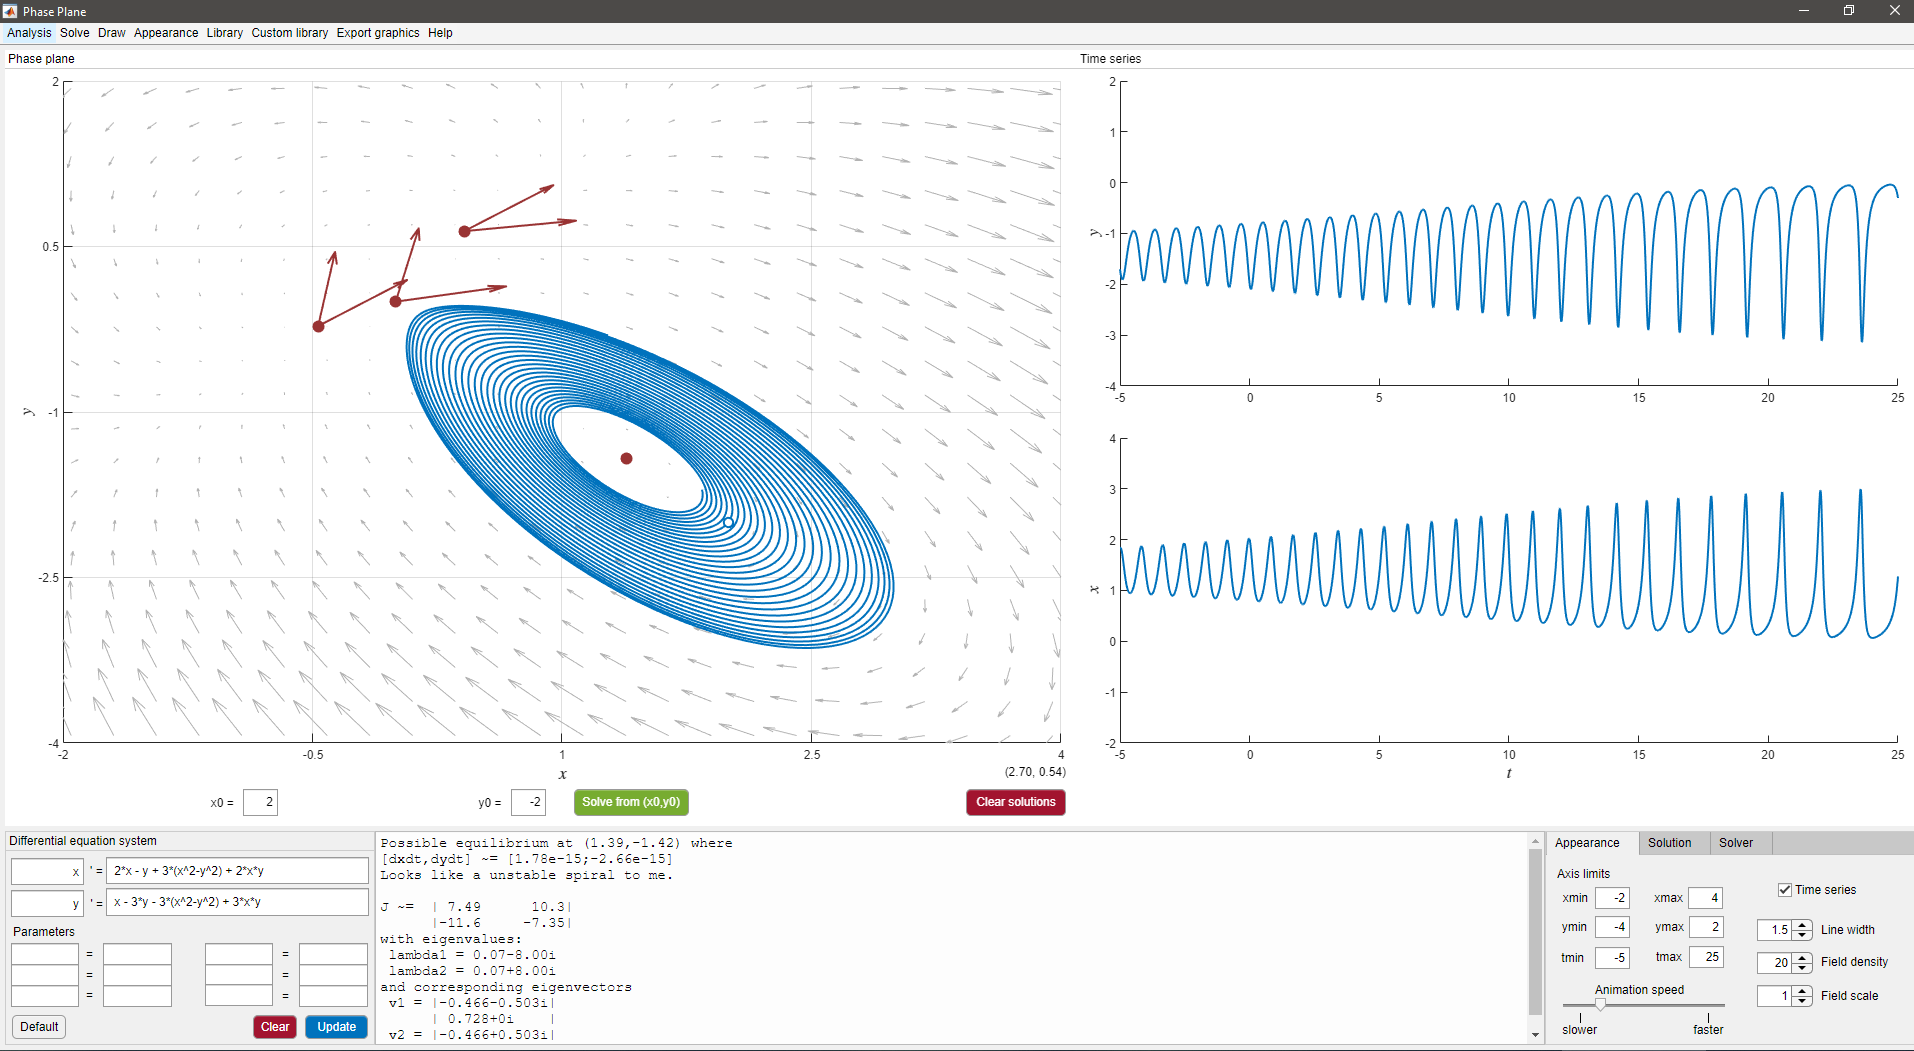
\includegraphics[width=16cm]{Project_App.png}
	\caption{The Phase Plane and Slope Fields App}
\end{figure}
Now we will go into detail and explain what every compartment does in the app.\\
The differential equations we will be using for this part are the following: 

\begin{displaymath}
 \frac{dx}{dt} = 2x-y+3(x^2-y^2)
\end{displaymath}
\begin{displaymath}
\frac{dy}{dt} = x-3y-3(x^2-y^2)+3xy
\end{displaymath}
\subsubsection{The Phase Plane}
The phase portrait shown below has initial conditions, $(x_0,y_0) = (2,-2)$. Once you have decided what your initial conditions will be you can go to the top left of the page and scan for any nearby equilibria. The app will start working a display any equilibrium it has found. As you can see in the figure below the differential equation has four equilibrium points, and their details will be on the bottom of the app which will be shown later.
\begin{figure}[H]
	\centering
	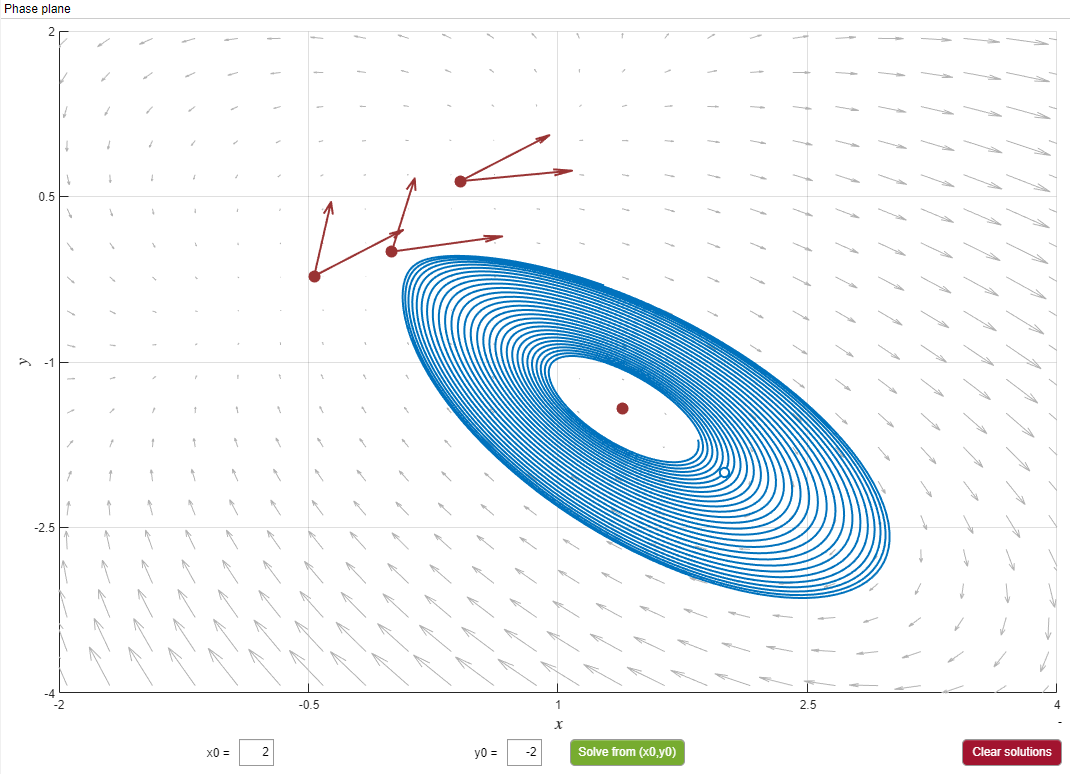
\includegraphics[width=  8cm]{Project_App_1.png}
	\caption{The Phase Plane $(x_0,y_0) = (2,-2)$}
\end{figure}
The app also gives you other options, for example it can display the nullclines of the differential equations which are not shown in the figure above but the app has this capability. Another option the app provides is that it allows the user to be able to display the eigenvectors it calculated when looking for the equilibrium points, that is why in the figure above we see arrows coming out of the equilibrium points found. 
\subsubsection{The Time Series}
The time series graphs allows us to see the how it function reacts with respect to time. For example as you can see below, the y vs t graph oscillates while also increasing in diameter of the graph and the x vs t graph does exactly the same thing. 
\begin{figure}[H]
	\centering
	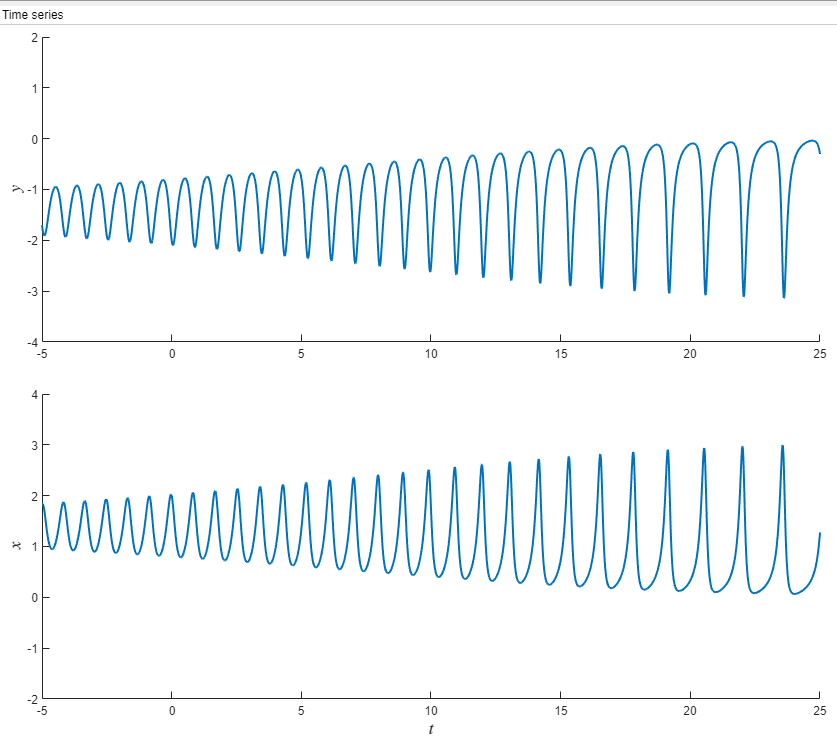
\includegraphics[width = 8cm]{Project_App_2.png}
	\caption{The Time Series}
\end{figure}
This is one of the reasons why we see a circular motion in the phase portrait, since the x vs t and y vs t graphs look like sine and cosine graphs we will get circles in the y vs x graph. 
\subsubsection{The Input, Equilibrium Details and Customization}
Finally we reach the place where all the magic begins.
\begin{figure}[H]
	\centering
	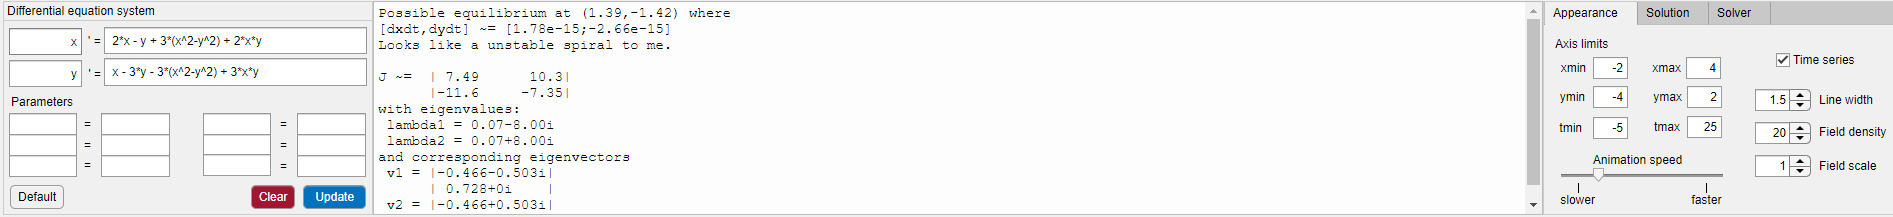
\includegraphics[width = 16cm]{Project_App_3.png}
	\caption{The Input, Equilibrium Details and Customization}
\end{figure}
On the left hand side is where the differential equations and their parameters are written in. Once you click the update button then the phase portrait is updated and begins to show the field vector that is created from the differential equations. In the center is where the user gets the info of the equilibrium point that they selected after scanning for equilibrium points. This is where the neat part of the app is, we get the coordinates of the equilibrium point, the stability, the corresponding Jacobian Matrix, the eigenvalues and its corresponding eigenvectors. Lastly, on the right hand side is where we get to customize how the graphs will look. This is where we update the x and y axis, and the t axis for the time series. Also, when you click on the other tabs the app allows to decide what ODE solver it will use to solve the ODE. 

\section{Results}
We were able to replicate the results from the use of MATLAB. The following pairs of phase plane diagrams will show the first diagram as result from MATLAB and the second from Browns use of Mathematica. Also the following phase plane diagrams will show the different cases for m and $\mu$.\\

\begin{figure}[H]
	\centering
	\begin{subfigure}[b]{0.4\textwidth}
		\centering
		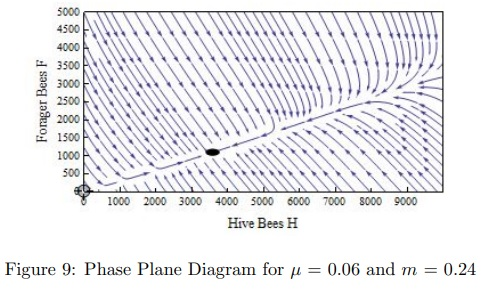
\includegraphics[width=5cm]{Figure_9_1.jpg}
		\caption{Brown's Figure\cite{Brown}}
	\end{subfigure}
	\hfill
	\begin{subfigure}[b]{0.4\textwidth}
		\centering
		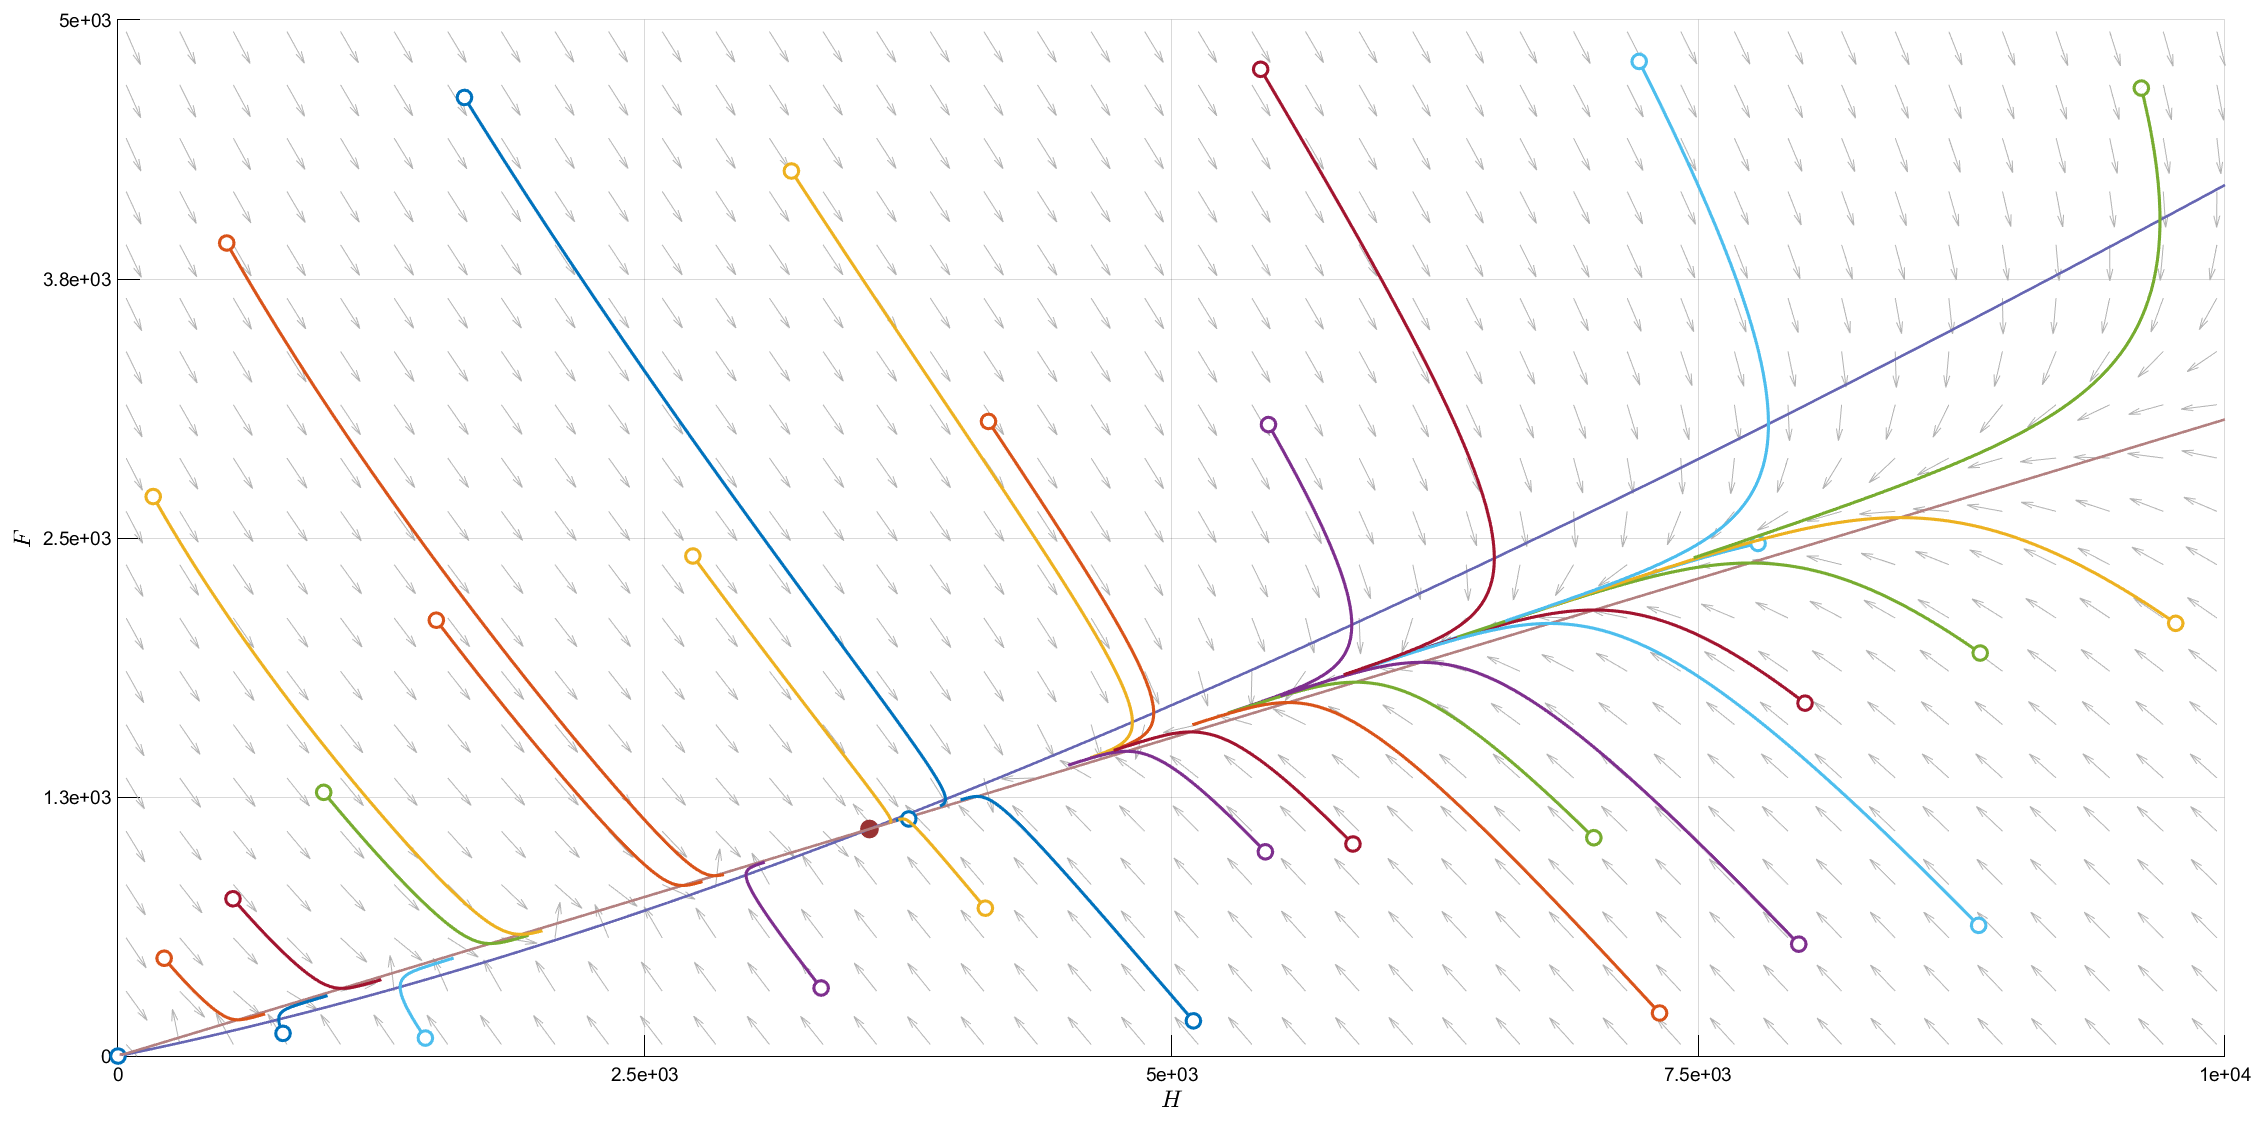
\includegraphics[width=5cm]{FIgure_1_M483_Phase.png}
		\caption{Our Figure}
	\end{subfigure}
	\begin{subfigure}[b]{0.4\textwidth}
		\centering
		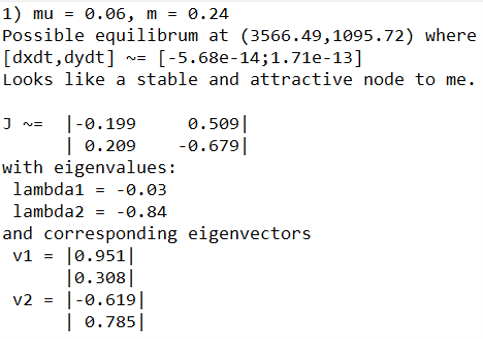
\includegraphics[width = 5cm]{Project_App_Info_1.png}
		\caption{Equilibrium Points and Their Details}
	\end{subfigure}
	\caption{$\mu = 0.06, m = 0.24$}
\end{figure}

\begin{figure}[H]
	\centering
	\begin{subfigure}[b]{0.4\textwidth}
		\centering
		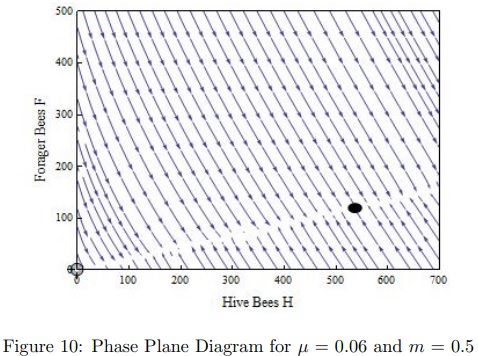
\includegraphics[width=4cm]{Figure_10_2.jpg}%
		\caption{Brown's Figure\cite{Brown}}
	\end{subfigure}
	\hfill
	\begin{subfigure}[b]{0.4\textwidth}
		\centering
		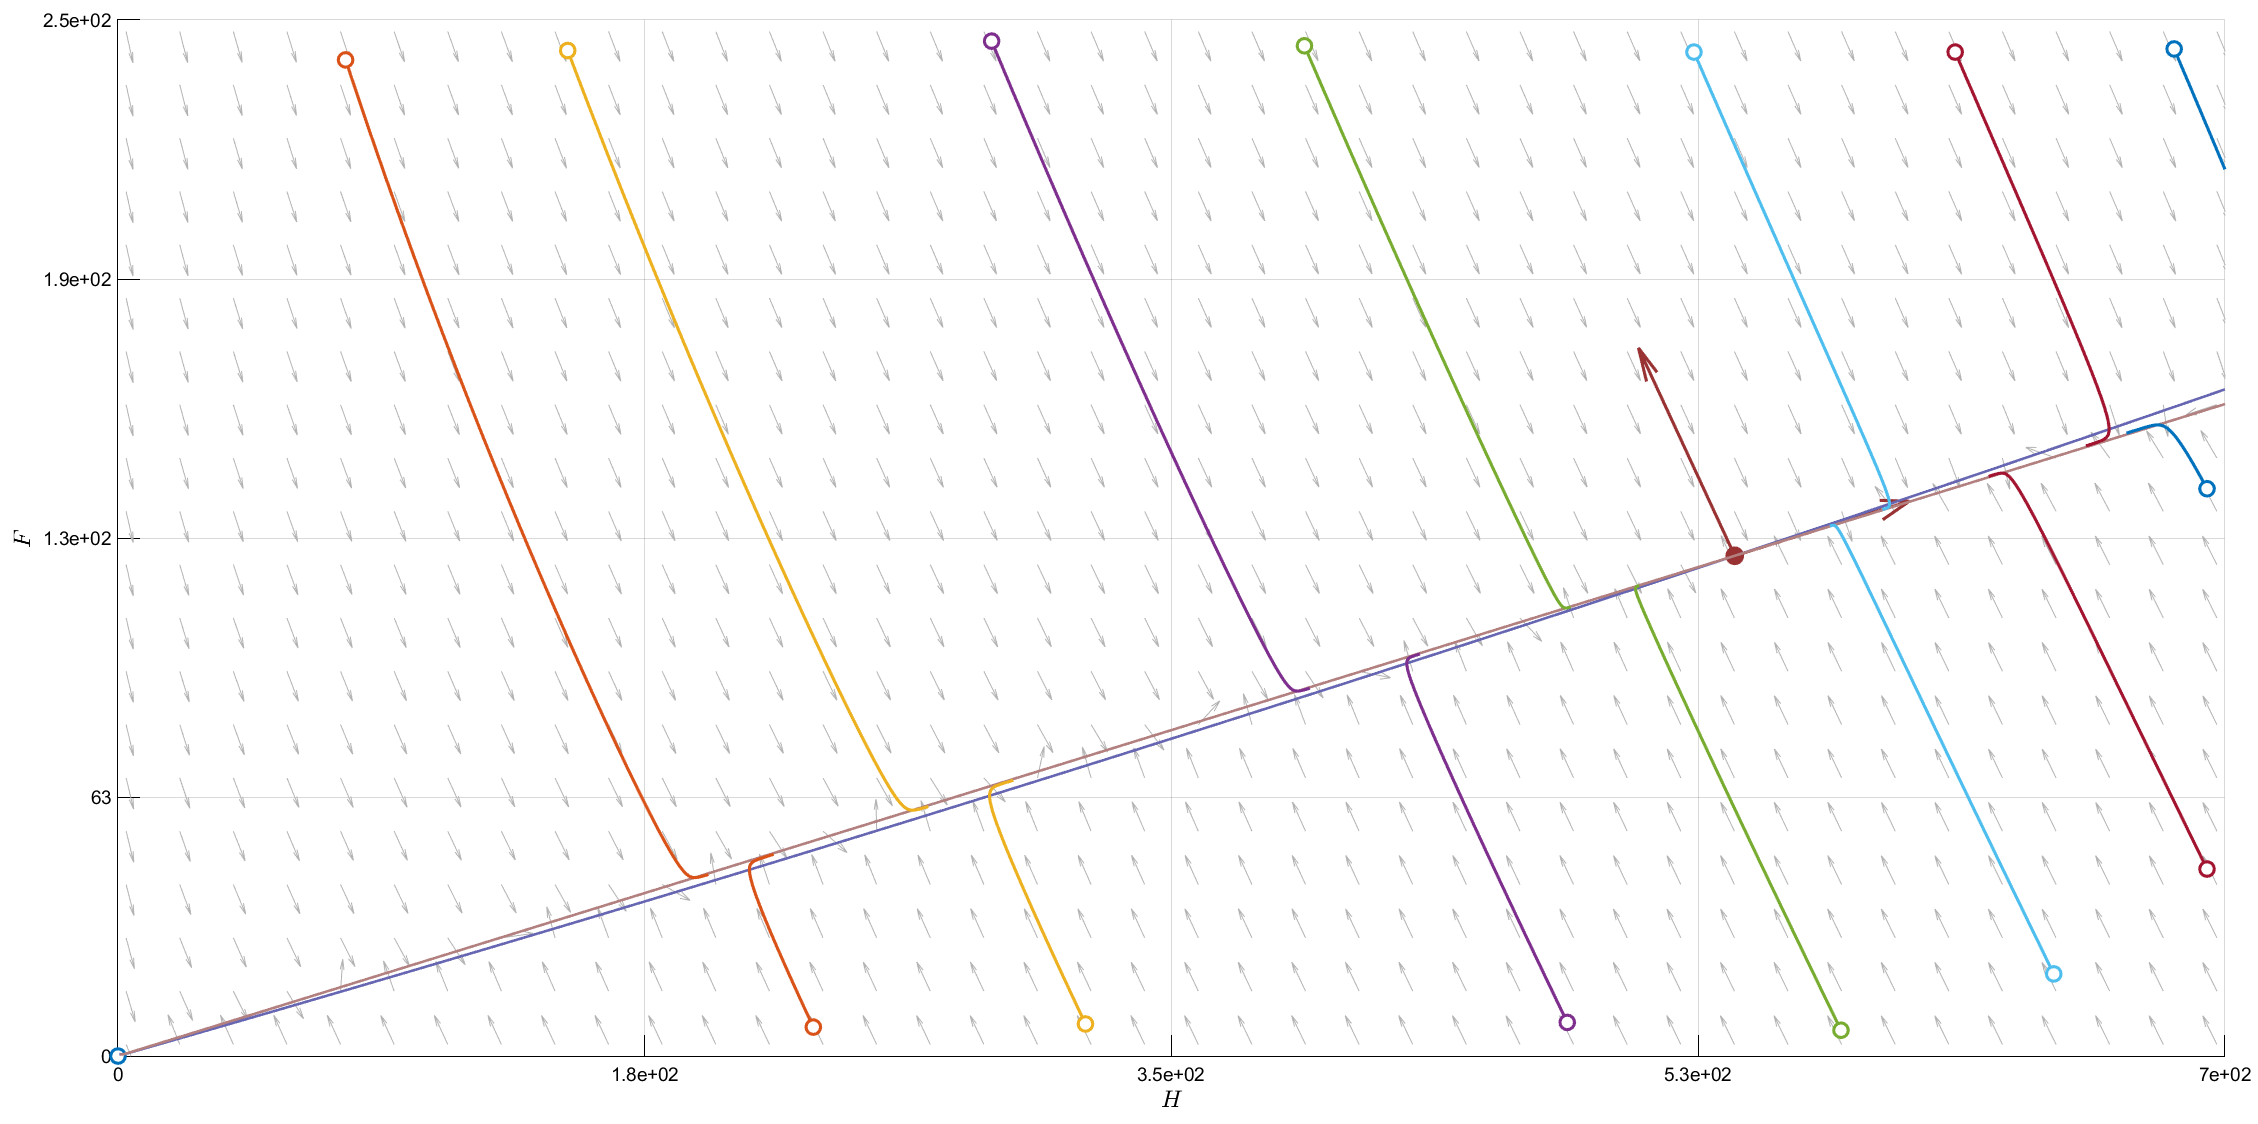
\includegraphics[width=4cm]{FIgure_2_M483_Phase.png}
		\caption{Our Figure}
	\end{subfigure}
	\begin{subfigure}[b]{0.4\textwidth}
		\centering
		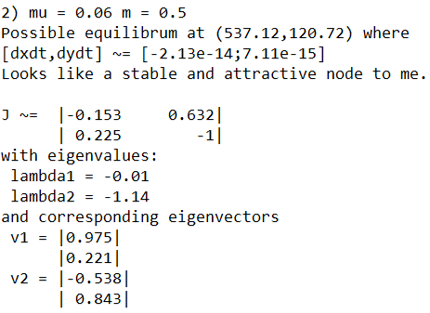
\includegraphics[width = 4cm]{Project_App_Info_2.png}
		\caption{Equilibrium Points and Their Details}
	\end{subfigure}
	\caption{$\mu = 0.06, m = 0.5$}
\end{figure}

\begin{figure}[H]
	\centering
	\begin{subfigure}[b]{0.4\textwidth}
		\centering
		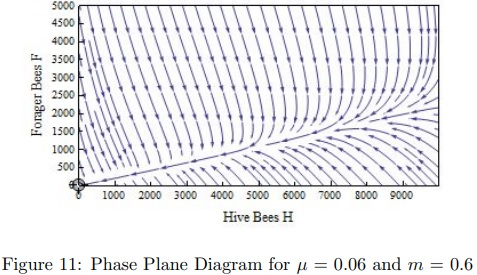
\includegraphics[width=5cm]{Figure_11_3.jpg}%
		\caption{Brown's Figure\cite{Brown}}
	\end{subfigure}
	\hfill
	\begin{subfigure}[b]{0.4\textwidth}
		\centering
		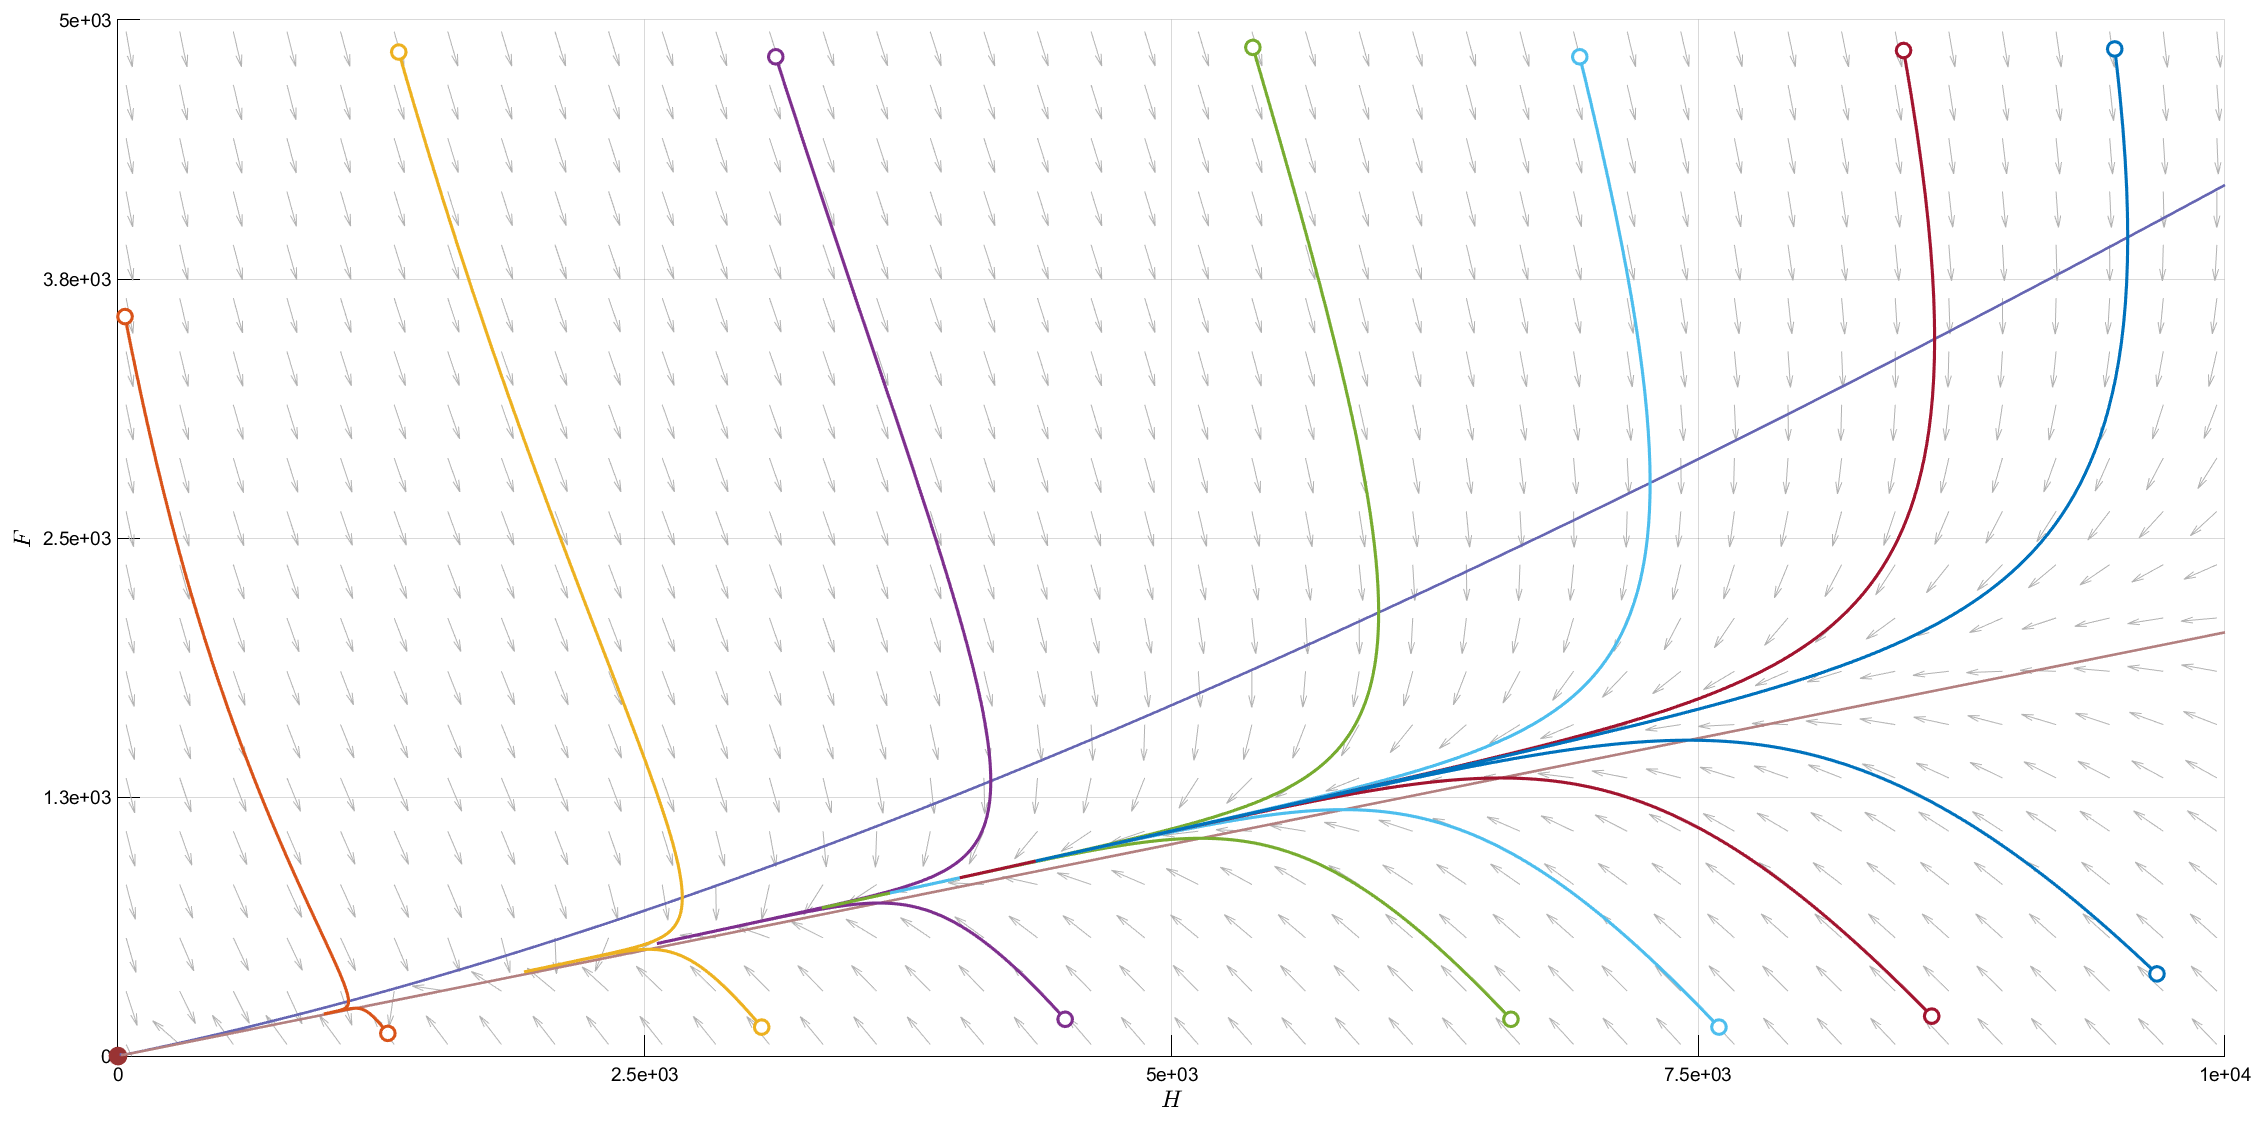
\includegraphics[width=5cm]{FIgure_3_M483_Phase.png}
		\caption{Our Figure}
	\end{subfigure}
	\begin{subfigure}[b]{0.4\textwidth}
		\centering
		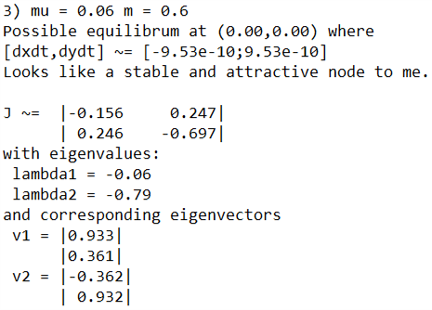
\includegraphics[width = 5cm]{Project_App_Info_3.png}
		\caption{Equilibrium Points and Their Details}
	\end{subfigure}
	\caption{$\mu = 0.06, m = 0.6$}
\end{figure}

\begin{figure}[H]
	\centering
	\begin{subfigure}[b]{0.4\textwidth}
		\centering
		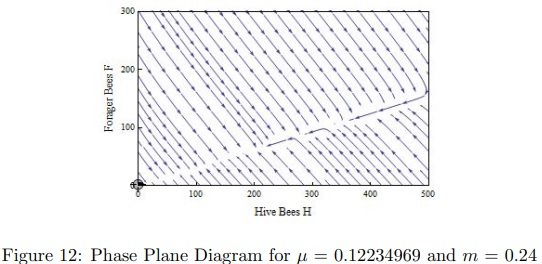
\includegraphics[width=5cm]{Figure_12_4.jpg}%
		\caption{Brown's Figure\cite{Brown}}
	\end{subfigure}
	\hfill
	\begin{subfigure}[b]{0.4\textwidth}
		\centering
		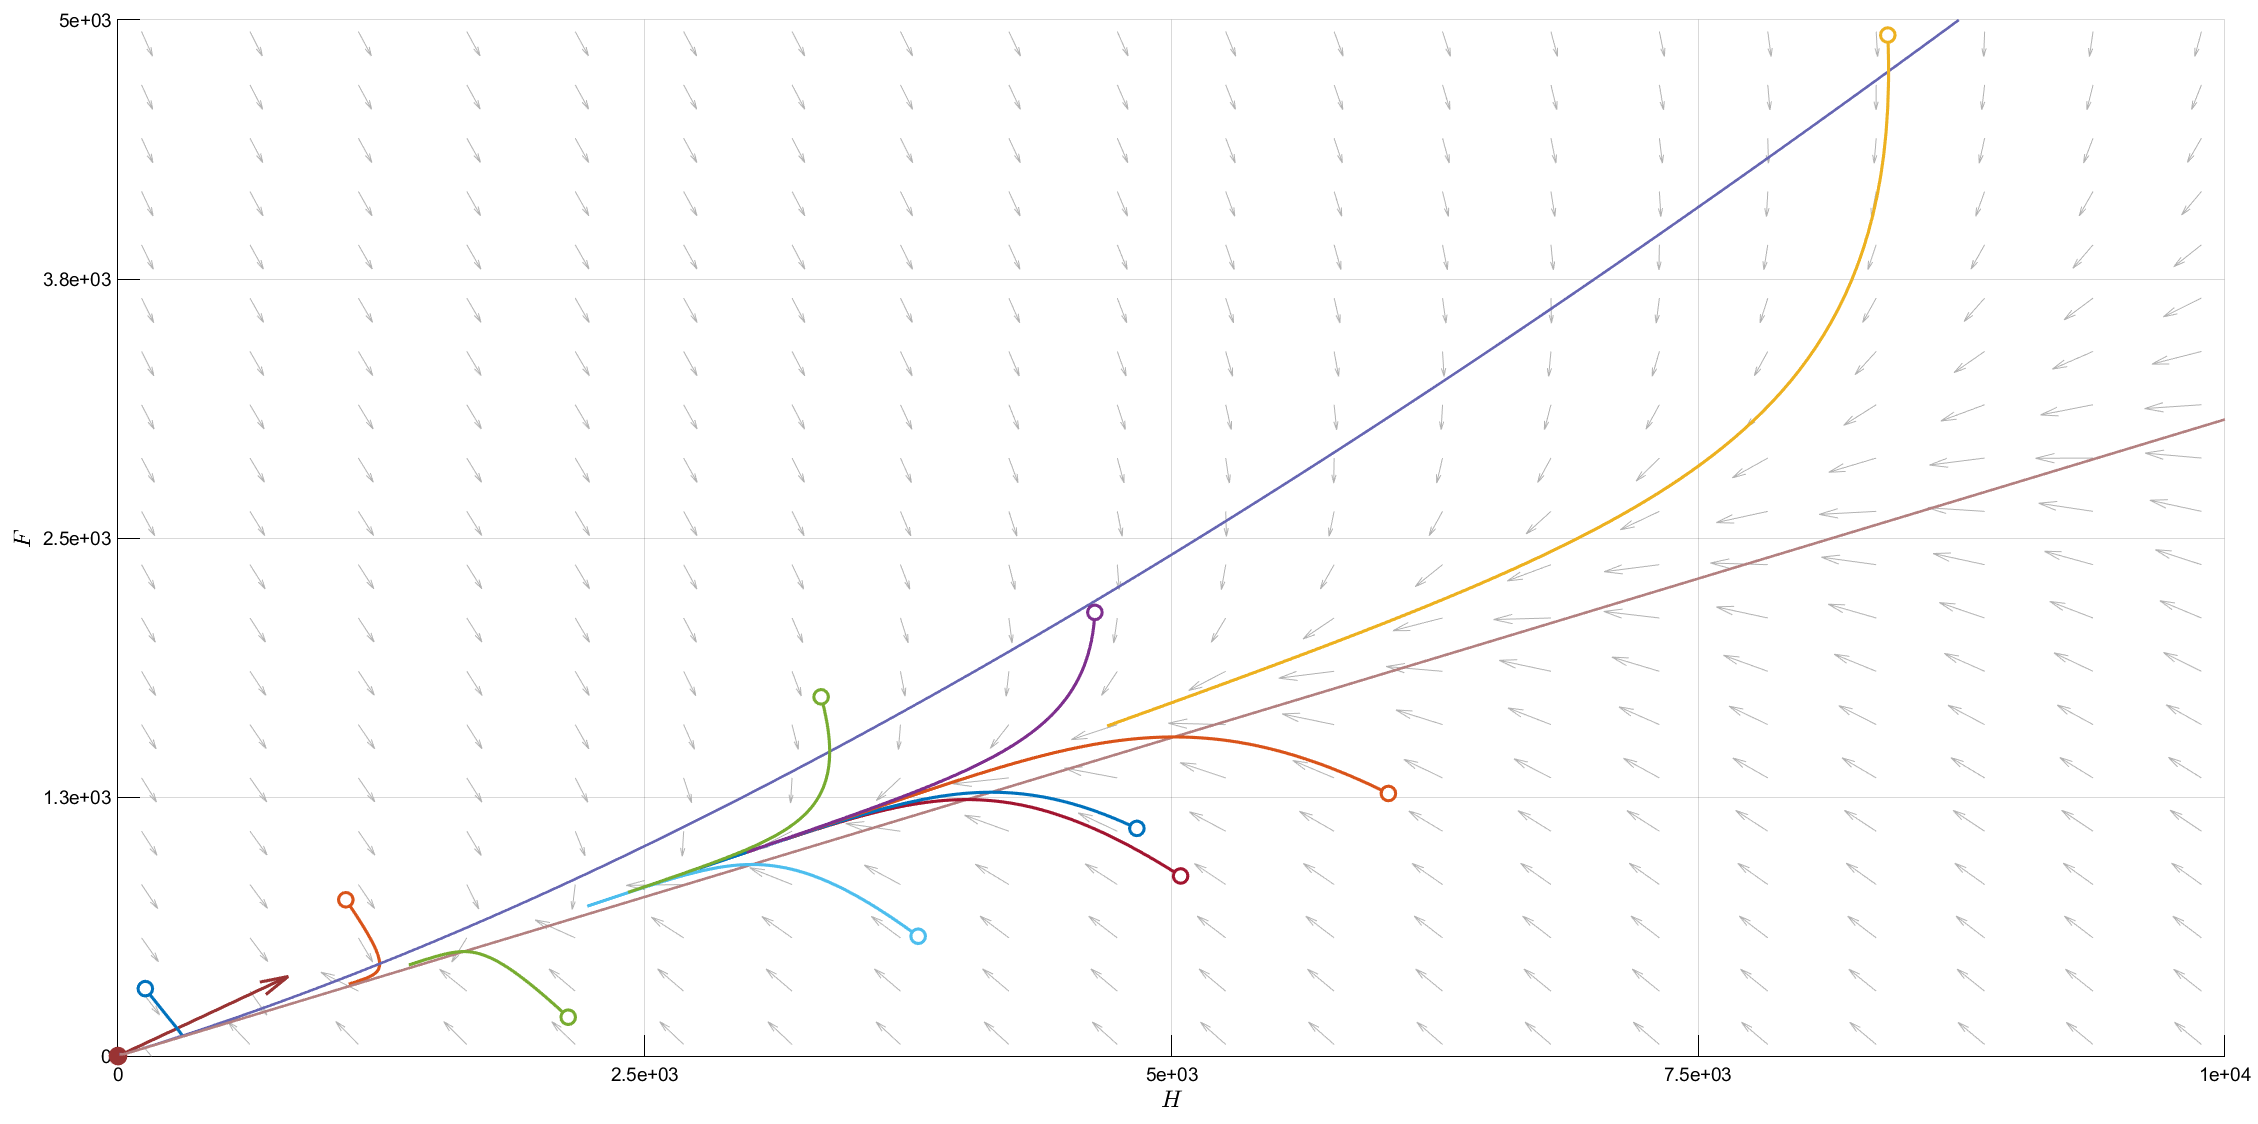
\includegraphics[width=5cm]{FIgure_4_M483_Phase.png}%
		\caption{Our Figure}
	\end{subfigure}
	\begin{subfigure}[b]{0.4\textwidth}
		\centering
		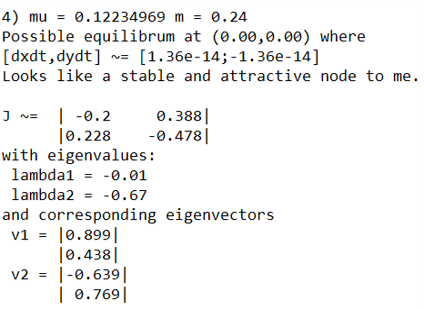
\includegraphics[width = 5cm]{Project_App_Info_4.png}
		\caption{Equilibrium Points and Their Details}
	\end{subfigure}
	\caption{$\mu = 0.12234969, m = 0.24$}
\end{figure}

\begin{figure}[H]
	\centering
	\begin{subfigure}[b]{0.4\textwidth}
		\centering
		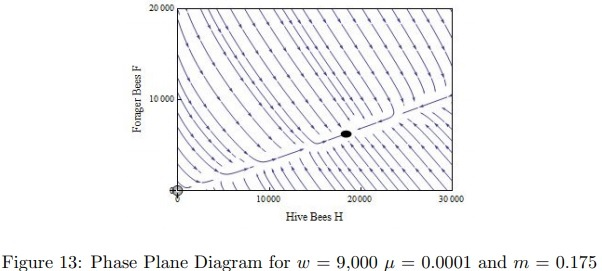
\includegraphics[width=6cm]{Figure_13_5.jpg}%
		\caption{Brown's Figure\cite{Brown}}
	\end{subfigure}
	\hfill
	\begin{subfigure}[b]{0.4\textwidth}
		\centering
		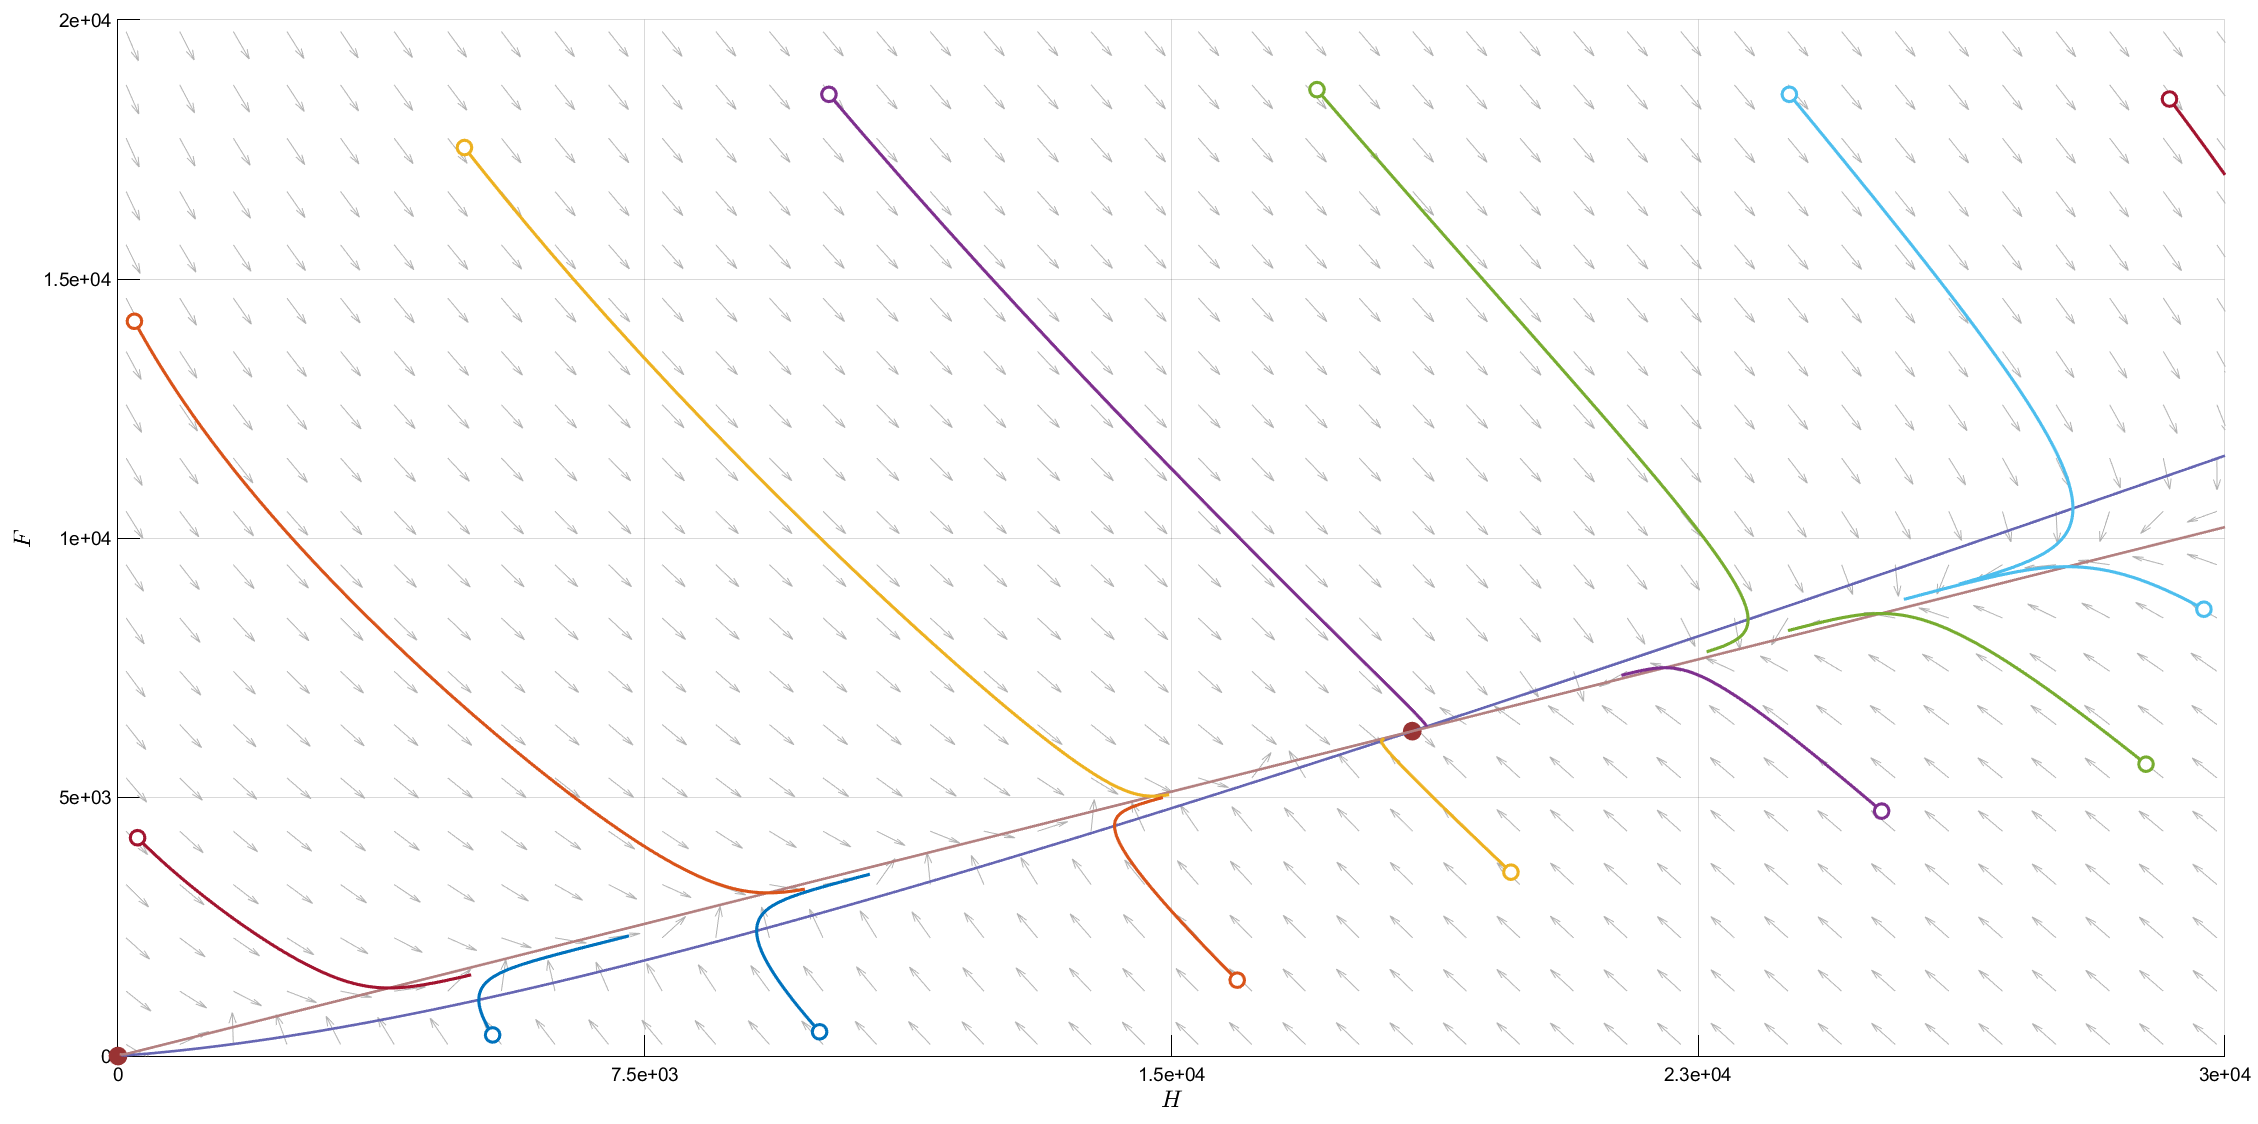
\includegraphics[width=6cm]{FIgure_5_M483_Phase.png}
		\caption{Our Figure}
	\end{subfigure}
\begin{subfigure}[b]{0.4\textwidth}
		\centering
		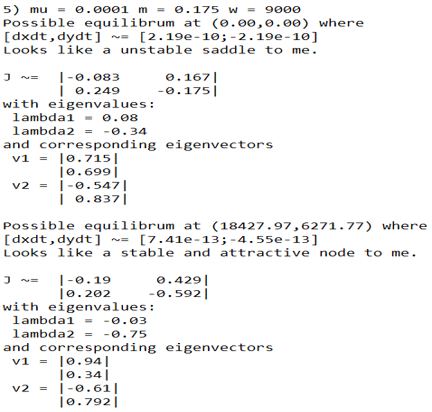
\includegraphics[width = 6cm]{Project_App_Info_5.png}
		\caption{Equilibrium Points and Their Details}
	\end{subfigure}
	\caption{$\mu = 0.0001, m = 0.175, \omega = 9000$}
\end{figure}

\section{Conclusion}
In conclusion, deriving the single colony model by Khoury, Myerscough and Barron 
leads to the use of two differential equations that explains the relations between hive bees and forager bee populations; where the model affects the forager bee death rate that leads 
to a colony's decline. Furthermore, Khoury presents a partition model that analyzes the 
impact of forager bee death rates within a colony's growth. Contributing factors to 
colony losses include viruses, mites, brood diseases, poor nutrition, pesticides, 
seasonal changes, migrating colonies for pollination season, and lastly the effect of 
food availability in colony growth.\\
 
Honey bees perform tasks that vary by age. Young hive bees carry out the safeguards within 
the hive while older adult forager bees execute dangerous duties outside the hive which include collecting pollen, nectar, and water. Foundational model from Khoury takes into account the hive bee population changes at a rate dependent from the arrival rate from pupae and the rate of transition to foragers. While the forager bee population changes at a rate that is dependent on the rate of transition from hive bees to their death rate. Additionally, Khoury regards the hive bee death rate to be small.\\

Brown has extended this model to improve some of the parameters that include a hive bee death rate with the addition of the parameter $\mu$. \cite{Seely}Assuming the per capita death rate of hive bees, $\mu$, is proportional to the number of hive bees. Also included are factors of pesticide contaminated  pollen in provisions and mites that would harmfully affect the hive bee death rate. In addition, the  improved model projects an existence of a positive stable equilibrium, where both hive and forager bees continue as the forager bee death rates are low. As levels exceed when forager death rates increase; honey bee colony collapses and is expected as both hive and forager bees drop to zero.\\

(w = emergence rate from brood to adult, L= daily laying rate of a queen)\\


In the original model, Khoury, Myerscough, and Barron \cite{Kho} used the parameter values w = 27,000 and L = 2000. For the Brown model, the value of w = 10,000 and L= 1500 was decreased to represent a realistic queen laying rate and the emergence rate according to Winston \cite{Winston}; in addition to adding a term to represent hive bee death rate. There are more factors  decreasing adult bee population, brood survivability must increase to balance, reflected in our model by a 
initial decrease in w. Realistically, however, it is difficult to increase brood survivability as the colony needs enough hive bees to feed the brood. Furthermore, maintaining an egg-laying rate of 1500 is difficult as the young hive bees clean out the brood cells for the eggs. There is an increased hive bee death rate that shuts down the queens egg-laying rate, if there were fewer hive bees to maintain the cells. 
To offset these harmful effects and achieve a desired larger colony population numbers by  reducing both the hive and forager bee death rates, brood survivability must increase. Based on  these results, we can conclude that smaller colony sizes occur, decreasing the colony's ability to carry its genes to the next generation.\\

Some improvements that could be made is to compare the predicted average lifespan by using raw experimental data and create a new model with different functions for the emergence rate from pupae and the transition rate to foraging. Also accounting for distance traveled for the forager bees journey to attain resources for their colony. Lastly, factoring for predation, meaning that foragers could be preyed upon when seeking resources and hives could be attacked from their nest.

\newpage
\addcontentsline{toc}{section}{References}
\begin{thebibliography}{}
\bibitem{Nowrski}Nowierski, Posted by Robert M., and R Hardy. "Pollinators at a Crossroads." USDA, United States Department of Agriculture, 24 June 2020, \begin{verbatim} www.usda.gov/media/blog/2020/06/24/pollinators-crossroads.\end{verbatim}
\bibitem{Kho}Khoury, David S, et al. "A Quantitative Model of Honey Bee Colony Population Dynamics." PLOS ONE, Public Library of Science , 18 Apr. 2011, \begin{verbatim}https://journals.plos.org/plosone/article?id=10.1371/journal.pone.0018491\end{verbatim}
\bibitem{Brown}Brown, Kelly M., "Mathematical Models of Honey Bee Populations: Rapid Population Decline." UMW Blogs, University of Mary Washington , Apr. 2013, \begin{verbatim} umwblogs.org/wp-content/blogs.dir/8053/files/2013/04/KellyBrownHonors.pdf. \end{verbatim}
\bibitem{Winston}Winston, Mark L. The Biology of the Honeybee. Harvard Univ. Press, 1995. 
\bibitem{Seely}Seeley, TD, The Wisdom of the Hive. Cambridge: Harvard University Press
\bibitem{Brian} Brian Hong,
\emph{Phase Plane and Slope Fields App}, MATLAB
\end{thebibliography}
\end{document}